\documentclass[a4paper]{scrartcl}
%\documentclass[a4paper]{report}

% Uncomment to optimize for double-sided printing.
% \KOMAoptions{twoside}

% Set binding correction manually, if known.
% \KOMAoptions{BCOR=2cm}

% Localization options
\usepackage[english]{babel}
\usepackage[T1]{fontenc}
\usepackage[utf8]{inputenc}

% Enhanced verbatim sections. We're mainly interested in
% \verbatiminput though.
\usepackage{verbatim}

% PDF-compatible landscape mode.
% Makes PDF viewers show the page rotated by 90°.
\usepackage{pdflscape}

% Advanced tables
\usepackage{tabu}
\usepackage{longtable}

% Fancy tablerules
\usepackage{booktabs}

% Graphics
\usepackage{graphicx}

% Current time
\usepackage[useregional=numeric]{datetime2}

% Float barriers.
% Automatically add a FloatBarrier to each \section
\usepackage[section]{placeins}

% Custom header and footer
% \usepackage{fancyhdr}
% \setlength{\headheight}{15.2pt}
% \pagestyle{fancyplain}

\usepackage{geometry}
\usepackage{layout}

\usepackage{subcaption}

% Math tools
\usepackage{mathtools}
% Math symbols
\usepackage{amsmath,amsfonts,amssymb}

% \fancyhf{}
% % Chapter header on non-plain pages only.
% \lhead{\fancyplain{} {\leftmark}}
% % Footer must contain print date. Ugly, but IPA requirement.
% \lfoot{\printdate}
% % Print date left and page count right was the thing which looked the
% % most balanced.
% \rfoot{\thepage}
% 
% Source code & highlighting
\usepackage{listings}

% Convenience commands
\newcommand{\mailsubject}{2419 - Computer Architecture - Series 1}
\newcommand{\maillink}[1]{\href{mailto:#1?subject=\mailsubject}
                               {#1}}

% Should use this command wherever the print date is mentioned.
\newcommand{\printdate}{\today}

\subject{2419 - Computer Architecture}
\title{Series 1, Theoretical Exercises}

\author{Michael Senn - 16-126-880\\ Pascal Gerig - 16-104-721}

\date{}

% Needs to be the last command in the preamble, for one reason or
% another. 
\usepackage{hyperref}


\begin{document}
\maketitle

% \tableofcontents

\section{String length}

The string \texttt{computer architecture} consists of 21 ASCII characters - as
such, those will account for 21 bytes on their own. In plain C the resulting
string will contain one additional byte at the end - the Null-byte which
indicates the end of the string. This adds up to a total of 22 bytes.

\section{Array access using pointers}

\subsection{Int array}

\begin{lstlisting}
int a[10];

int getAt(int i) {
        return a[i];
}

int getAt(int *a, int i) {
        return *(a+i);
}
\end{lstlisting}


\subsection{Char array}


\begin{lstlisting}
char a[10];

char getAt(int i) {
        return a[i];
}

char getAt(char *a, int i) {
        return *(a+i);
}
\end{lstlisting}

\subsection{Explanation}

The pointer-arithmetic based function uses the fact that adding an integer i to
a pointer p will return the memory address i * n ahead of p, with n being the
size of the data type which p points to.

As such, this can be used to retrieve the array element at position p+i, given
an initial (pointer to) element p, and an offset i.

\section{Pointer types}

For the purpose of this exercise we'll assume the size of a long to be 4 bytes
- even though its size on 64-bit versions of Linux and Mac OS is 8 bytes.

The output as a whole - with detailed explanations below - will be:

\begin{lstlisting}
bffff604
3b9aca00
ca
9a
bffff607
\end{lstlisting}


\subsection{Walkthrough}

\begin{lstlisting}
void * p = &b;
\end{lstlisting}

Having declared \texttt{p} as a void pointer, pointing to the memory address of
the first byte of \texttt{b}, \texttt{p} will be equal to \texttt{bffff604}.

\begin{lstlisting}
printf("%x\n", p);
\end{lstlisting}

Printing the value of \texttt{p} in hexadecimal format will print out
\texttt{bffff604}.

\begin{lstlisting}
printf("%x\n", *(long*)p++);
\end{lstlisting}

It should be noted that \texttt{p++} will evaluate to the value of p before incrementation.

As such it will cast the void pointer to a long pointer, dereference it
accessing the 4-byte memory block starting at \texttt{bffff604}, treat that as
a long, then print it.

This will lead to \texttt{3b9aca00} being printed.

\texttt{p} will now - due to being a void pointer and having been incremented
by one - point at \texttt{bffff605}.

\begin{lstlisting}
printf("%x\n", *(char*)p++);
\end{lstlisting}

Similar to the above, this will access the one-byte memory block starting at
\texttt{bffff605}, and print its hexadecimally-formatted value.

Hence it will print \texttt{ca}.

It should be noted that, due to a char being a signed one-byte integer, the
value of said char would actually be \texttt{-54}. 

\texttt{p} will now point at {bffff606}.

\begin{lstlisting}
printf("%x\n", *(unsigned char*)p++);
\end{lstlisting}

Once more we access the one-byte memory block starting at \texttt{bffff606} and
print it.

\texttt{9a}.

\texttt{p} will now point at \texttt{bffff607}.

\begin{lstlisting}
printf("%x\n", p);
\end{lstlisting}

Lastly we print the memory address which \texttt{p} points to currently:
\texttt{bffff607}.

\section{Parameter passing}

In both versions, \texttt{i} will be incremented by one, and therefore have the
value \texttt{104}. The difference lies in what happens to \texttt{j}. In the
first version the already-incremented value will be returned by the function,
and \texttt{j} therefore be \texttt{104} as well. Wheras in the second version,
the not-yet-incremented value will be returned, leaving \texttt{j} as
\texttt{103}.

\section{Pointer arithmetic}

In the first program, both \texttt{x} and \texttt{px} will initially point at
the array's first element. Afterwards, \texttt{px} is incremented by one,
therefore pointing at the array's second element.

Hence, the output will be

\begin{lstlisting}
3 3
3 2
\end{lstlisting}

In the second program, the value at the location of \texttt{px} - which is the
same location which \texttt{x} points to - is changed to \texttt{20},
\texttt{px} decremented, and the value at its new location changed to
\texttt{21}. As such, the output will be \texttt{20 21}.

The issue here is that the location "one char left of x" is unassigned memory
within the current scope. As such, we might be unintentionally modifying data
used in other parts of our program, or simply crash if we happen to access a
memory block which is outside the range the OS allocated to us.


\section{Structs and Unions}

For the purpose of this exercise we'll assume chars to be one, shorts to be
two, and ints to be four, bytes long.

As such, the defined struct contains one 10-byte char array, two one-byte
chars, and one two-byte short, adding up to a total of \texttt{10 + 1 + 1 + 2 =
14} bytes.

The defined union - within which the various variables will overlap insofar as they
all start at the same location in memory - will therefore have its length defined by its
longest member, the 12-byte char array, for a total length of \texttt{12}
bytes.

As such, the output (due to lack of newlines in the printf format string) will be \texttt{1412}.

\begin{figure}
	\centering
	\textbf{Memory layout of struct and union}\par\medskip
	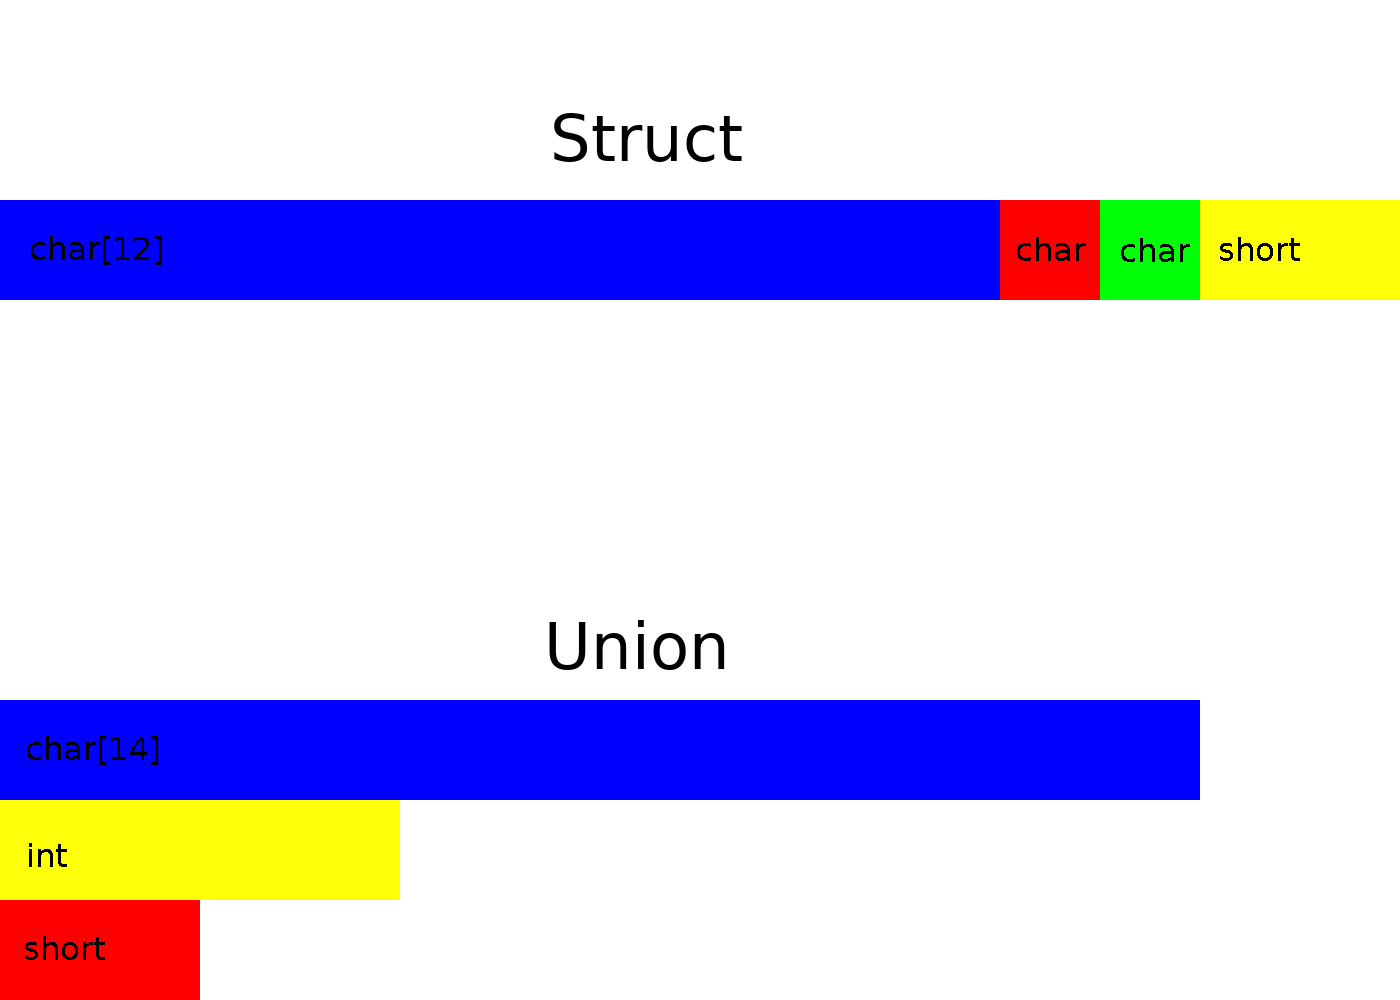
\includegraphics[width=\textwidth]{resources/memory_layout.png}
\end{figure}

\section{Define}

Define works by creating an 'alias' for a given expression. All occurences of
that alias will then be replaced by its definition by the preprocessor.

As such, the program's output will be \texttt{15} - that is, if it wouldn't
refuse to compile due to an undefined \texttt{EXIT\_SUCCESS}.

\end{document}
